\documentclass[12pt, a4paper]{report}
\usepackage[utf8]{inputenc}
\newcommand\preamble{
    \usepackage[italian]{babel}
    \usepackage{geometry}
    \usepackage{amsmath}
    \usepackage{amssymb}
    \usepackage{graphicx}
    \usepackage{ulem}
    \usepackage{amsthm}
    \theoremstyle{definition}
    \newtheorem{definition}{Def}[section]
    \usepackage{listings}
    \usepackage{xparse}
    \usepackage{expl3}
    \usepackage{tikz}
    \usepackage{xcolor}
    \definecolor{codegreen}{rgb}{0,0.6,0}
    \definecolor{codegray}{rgb}{0.5,0.5,0.5}
    \definecolor{codepurple}{rgb}{0.58,0,0.82}
    \definecolor{backcolour}{rgb}{0.95,0.95,0.92}

    \lstdefinestyle{mystyle}{
        backgroundcolor=\color{backcolour},   
        commentstyle=\color{codegreen},
        keywordstyle=\color{magenta},
        numberstyle=\tiny\color{codegray},
        stringstyle=\color{codepurple},
        basicstyle=\ttfamily\footnotesize,
        breakatwhitespace=false,         
        breaklines=true,                 
        captionpos=b,                    
        keepspaces=true,                 
        numbers=left,                    
        numbersep=5pt,                  
        showspaces=false,                
        showstringspaces=false,
        showtabs=false,                  
        tabsize=2
    }

    \lstset{style=mystyle}
    \usepackage[colorlinks=true, linkcolor=blue]{hyperref}
    \usetikzlibrary{calc}
    \let\olditemize\itemize
    \renewcommand\itemize{\olditemize\setlength\itemsep{0em}}
    \geometry{a4paper, left=1.2cm, right=1cm, top=1cm, bottom=2cm}
}
\newcommand{\tikzmark}[1]{\tikz[baseline,remember picture] \coordinate (#1) {};}
\newcommand{\customfbox}[1]{
    \begin{center}
        \noindent\fbox{\parbox{\dimexpr\linewidth-2\fboxsep-2\fboxrule\relax}{\centering #1}}
    \end{center}
    }
\newcommand{\imagePath}{Images/logoUni.png}

\newcommand{\customTitlePage}[5]{
    \newcommand{\courseTitle}{#1}
    \newcommand{\authorName}{#2}
    \newcommand{\academicYear}{#3}
    \newcommand{\universityName}{#4}
    
    \begin{titlepage}
        \centering
        \includegraphics[width=0.5\textwidth]{\imagePath}\par\vspace{1cm}
        {\scshape\LARGE \universityName \par}
        \vspace{1.5cm}
        {\huge\bfseries \courseTitle \par}
        \vspace{2cm}
        {\Large\itshape \authorName \par}
        \vfill
        \academicYear
    \end{titlepage}
}
\preamble

\begin{document}
    \customTitlePage{Programmazione Concorrente Algoritmi Distribuiti}{Lorenzo Vaccarecci}{Anno Accademico 2024/2025}{Università degli Studi di Genova}
    \newpage
    \tableofcontents
    \chapter{Introduzione}
        \section{Perchè usare/sviluppare sistemi concorrenti/distribuiti?}
            Perchè in questo modo siamo più efficienti, distribuiamo dei dati, condividiamo delle risorse, usiamo reti di computer e per comunicare.
        \section{Perchè è difficile concettualmente?}
            Perchè se ho $n$ processi e $m$ istruzioni per processo, ho
            \begin{equation*}
                \frac{(n\cdot m)!}{(m!)^{n}}
            \end{equation*}
            possibili "percorsi" che un'esecuzione concorrente/distribuita può avere.
        \section{Programma concorrente}
            E' un insieme di processi che si eseguono in parallelo (programmi che si eseguono su processori diversi ma anche programmi multi-task che si eseguono sullo stesso processore dando l'illusione del parallelismo) e che comunicano (scambio di dati tramite messaggi o memoria condivisa che permette la sincronizzazione).
        \section{Esecuzione concorrente}
            L'esecuzione di un programma concorrente è composto da un insieme di processi ciascuno dei quali dispone di un insieme di istruzioni atomiche. Ogni processo ha un puntatore verso la prossima istruzione da eseguire e l'esecuzione del programma concorrente è un intreccio arbitrario delle istruzioni dei vari processi (interleaving), la prossima istruzione è dunque scelta fra quelle puntate dai vari processori: tanti possibili scenari (1.2).
        \section{Comunicazione via memoria condivisa}
            I processi hanno un accesso comune alla memoria che può essere tramite variabile condivisa o con strutture più complesse. Se si usa una variabile condivisa deve essere possibile scrivere e leggere e bisogna fare attenzione alla gestione dell'accesso (se transazione atomica o non atomica). Ci sono vari casi possibili:
            \begin{itemize}
                \item \textbf{Multiple Reader/Multiple Writer}
                \item \textbf{Multiple Reader/Single Writer}
            \end{itemize}
    \chapter{Processi e Thread}
        \section{Processi}
            Un processo è un programma in corso di esecuzione. Ogni processo necessita di uno spazio di indirizzamento dedicato (stack) e di input e output. \\
            Più processi possono essere eseguiti sulla stessa macchina in un modo quasi simultaneo, un processo non ha accesso allo spazio di indirizzamento degli altri e permette di avere un'illusione di parallelismo.
            \subsection{Unix}
                \subsubsection{Creazione di un processo}
                    \begin{center}
                        \texttt{pid\_t fork(void);}
                    \end{center}
                    Ritorna 0 al figlio e il PID del figlio al padre. \\
                    \texttt{fork()} crea un processo figlio che è una copia esatta del padre, con lo stesso codice, dati e spazio di indirizzamento. Le variabili non sono condivise.
                    \begin{center}
                        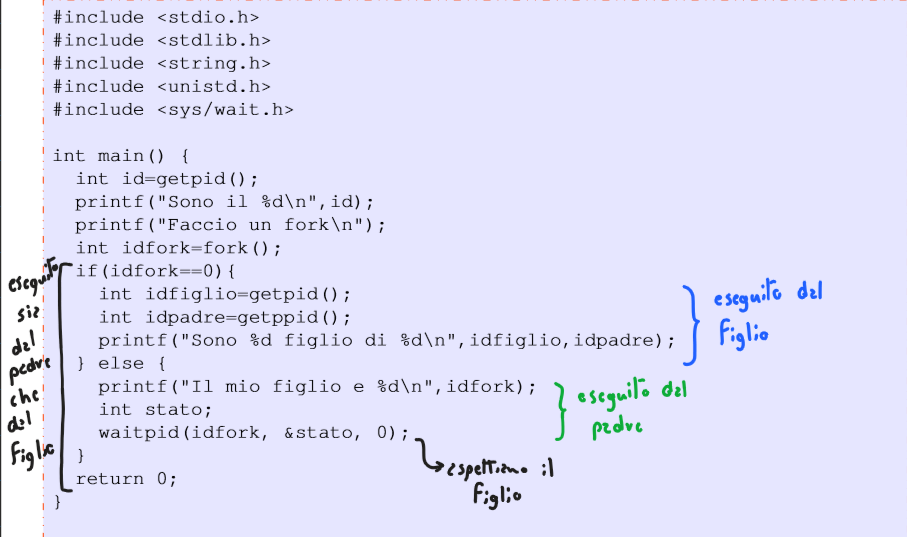
\includegraphics[width=0.8\textwidth]{Images/fork.png}
                    \end{center}
                \subsubsection{Esecuzione di un comando}
                    \begin{center}
                        \texttt{int execvp(const char *file, char *const argv[]);}
                    \end{center}
                    Dove \texttt{file} è il nomde del comando che vogliamo eseguire e l'array \texttt{argv} contiene: 
                    \begin{itemize}
                        \item Il nome del comando nel primo campo
                        \item Gli argomenti del comando
                        \item \texttt{NULL} per indicare la fine dell'array in posizione finale \underline{obbligatoria}
                    \end{itemize}
            \subsection{Pipe}
                Servono per la comunicazione fra processi. Le pipes sono dei canali unidirezionali considerati come dei descrittori di file.
                \begin{center}
                    
\includegraphics[width=0.7\textwidth]{Images/pipe.png}
                \end{center}
                \begin{center}
                    \texttt{int pipe(int fd[2]);}
                \end{center}
                Dove \texttt{fd[0]} è il descrittore di lettura e \texttt{fd[1]} è il descrittore di scrittura. Dopo il forkk, entrambi i  processi possono scrivere e leggere ma perchè funzioni bisogna chiudere il descrittore che non si usa.
        \section{Thread}
            Un thread è un filo d'esecuzione dentro un programma, è eseguito da un processo e possono esserci più thread in un processo (processo multi-thread). Ogni thread è diverso e ha come attributi: \begin{itemize}
                \item Un puntatore di esecuzione o \texttt{PC} (Program Counter)
                \item Uno stack
            \end{itemize}
            \subsection{POSIX}
                \begin{center}
                    \texttt{\#include <pthread.h>}
                \end{center}
                Bisogna anche dire al momento della compilazione che si desidera usare questa libreria con il flag \texttt{-pthread} o \texttt{-lpthread}.
                \subsubsection{Creazione di un thread}
                    \begin{center}
                        \texttt{int pthread\_create(pthread\_t *thread, const pthread\_attr\_t *attr, void *(*start\_routine) (void *), void *arg);}
                    \end{center}
                    Per condividere le variabili si usa la keyword \texttt{volatile}.
                \subsubsection{Locks}
                    L'accesso ai dati condivisi deve essere protetto:
                    \begin{itemize}
                        \item Un thread che desidera accedere a un dato condiviso richiede il lock
                        \item Se il lock è libero, prosegue altrimento rimaane bloccato finchè il lock non è libero
                        \item Quando ha finito, rilascia il lock
                    \end{itemize}
                    Questi lock sono condivisi tra i threads.\\
                    E' buona pratica far liberare il lock dal thread che lo ha preso.
                    \begin{center}
                        \texttt{pthread\_mutex\_t lock = PTHREAD\_MUTEX\_INITIALIZER;}\\
                        \texttt{int pthread\_mutex\_lock(pthread\_mutex\_t *mutex)}\\
                        \texttt{int pthread\_mutex\_unlock(pthread\_mutex\_t *mutex)}
                    \end{center}
                    Queste due funzioni ritornano 0 se tutto è andato a buon fine.
    \chapter{Interleaving e Mutua esclusione}
        \section{Istruzioni atomiche}
            Un'istruzione atomica è eseguita completamente senza essere interrotta, in questo corso supponiamo che ogni riga nei programmi sarà atomica.
            \begin{lstlisting}[language=C]
            x = x + 1;
            if(x == 2) { // Questo if potrebbe essere interrotto e x potrebbe cambiare
                x = 3;
            }
            \end{lstlisting}
        \section{Ipotesi di atomicità}
            \customfbox{Le ipotesi possono cambiare a seconda del compilatore, il processore, ecc.}
            \textbf{Evitare di scrivere istruzioni che manipolano più di una volta la stessa variabile condivisa tra più processi o thread senza un'adeguata sincronizzazione.}
            \begin{itemize}
                \item \textbf{Registri atomici}: operazione di lettura e di scrittura atomiche
                \item \textbf{Test-and-set}: si può testaare e modificare una variabile senza essere interrotto
                \item \textbf{Swap}: si può cambiare il valore di un registro locale e di uno condiviso in modo atomico.
                \item \ldots
            \end{itemize}
        \section{Interleaving}
            \customfbox{
                \begin{definition}
                    Uno stato di un programma concorrente $P$ è una tupla con: \begin{itemize}
                        \item un puntatore d'istruzioni per ciascun processo
                        \item un valore per ciascuna variabile (locale o condivisa)
                    \end{itemize}
                \end{definition}
            }
            \customfbox{
                \begin{definition}
                    Per due stati $s_{1}$ e $s_{2}$ si scrive $s_{1}\rightarrow s_{2}$ quando si può passare da $s_{1}$ a $s_{2}$ usando una delle istruzioni puntata in $s_{1}$.
                \end{definition}
            }
            \customfbox{
                \begin{definition}
                    Il diagramma degli stati di $P$ è il sistema di transizione $TS_{P}=(S,\rightarrow,s_{0})$ dove:
                    \begin{itemize}
                        \item $S$ è l'insieme degli stati di $P$
                        \item $s_{0}$ è lo stato iniziale di $P$
                        \item $\rightarrow$ è la relazione di transizione inclusa in $S \times S$
                    \end{itemize}
                    Un cammmino in $TS_{P}$ è uno scenario possibile per $P$.
                \end{definition}
            }
            \begin{center}
                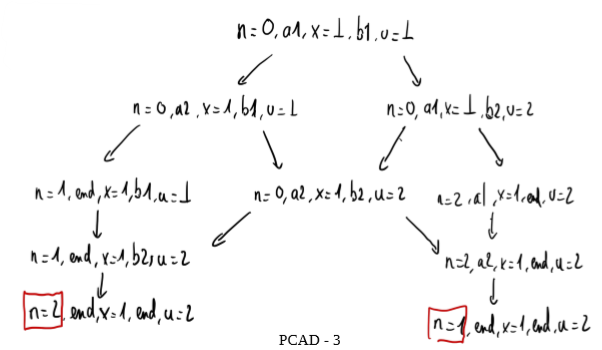
\includegraphics[width=0.6\textwidth]{Images/tsp.png}
            \end{center}
            I cammini in $TS_{P}$ corrispondono a tutti gli intrecci possibili per $P$. Facciamo quindi l'ipotesi che tutti questi intrecci siano possibili.
                \subsection{Semantica ragionevole}
                    \begin{itemize}
                        \item \textbf{Sistemi con un processore}: c'è una successione d'istruzioni
                        \item \textbf{Sistemi con più processori}: ogni processo è legato a un processore e l'interleaving non corrisponde esattamente alla realtà (azioni parallele), ma è corretta se non ci sono conflitti sulle risorse.
                        \item \textbf{Sistemi distribuiti}: diversi computer, nessuna variabile condivisa, comunicazione tramite messaggi. Molto diversa rispetto ai primi due casi, ma la semantica rimane interessante se uno ci aggiunge l'invio e la ricezione di messaggi.
                    \end{itemize}
            \section{Mutua esclusione}
\end{document}